% Provenance (never printed): see sources/outline_sources.md (Year 2: energy geology --- the
% petroleum system quantified, unconventional resources, geothermal systems, uranium deposits,
% geological storage of carbon dioxide).
% Kerogen kinetics and elemental analyses: Fletcher and Pugmire (DOE, OSTI 1176871); kerogen
% types and Easy%Ro: Advanced Chemistry Basins Project (DOE, OSTI 830009); maturity thresholds:
% USGS MF-2008-B; TTI: Waples (1980) and Hammerschmidt et al. (2014); volumetrics and CO2
% storage: DOE/NETL (2008) and IPCC SRCCS (2005) chapter 5; geothermal: USGS OFR 2008-1296 and
% FS 2008-3082; uranium: USGS Bulletin 1693; Oklo: OSTI abstract records. Ledger rows in
% sources/ledger/book4.md; curves from figdata/bachelor-2/maturation.py and co2_density.py,
% numbers from the Book 4 second-writer scratch calculator calc/ch30.py.
% Geology and sourced numbers only: no advocacy, no policy.
\chapter{Energy Geology}\label{ch:b2:energy-geology}

Oil is the remains of microscopic organisms, buried with mud and cooked for millions of years at
around \qty{100}{\celsius}; geothermal energy is the same warmth of the Earth, taken directly.
Both are ruled by temperature and time: the first by the rate at which a chemical reaction runs as
buried rocks slowly warm, the second by how much heat a volume of rock stores and how fast water
can carry it to a well. This chapter quantifies the petroleum system, turns to the resources that
lack one of its elements, to geothermal heat and to uranium, and ends with the reverse operation:
putting carbon dioxide back underground.
% ledger: earle:oil-window, earle:organic-preservation

\begin{recall}
\textbf{From the school volumes}: source rock, kerogen, maturation, oil window, migration,
reservoir rock, seal, trap, overburden, petroleum system; coal and coal rank; geothermal energy.
\textbf{From the Year 1 volume}: heat flow and the geotherm; porosity and permeability; pore-fluid
pressure, effective stress and the Coulomb criterion; borehole log; sedimentary basin and
subsidence. \textbf{From the chemistry books}: the Arrhenius law, activation energy, first-order
reaction. \textbf{From the physics books}: radioactive decay, decay constant, half-life; the
critical point of a fluid. \textbf{From \cref{ch:b2:basins-compared}}: \omterm{def:b2:basins-compared:curve}{subsidence curve}.
\textbf{From \cref{ch:b2:ore-deposits}}: \omterm{def:b2:ore-deposits:types}{ore-deposit type}, \omterm{def:b2:ore-deposits:grade}{tonnage}.
\end{recall}

\section{The petroleum system quantified}\label{sec:b2:energy-geology:petroleum}

A petroleum system needs a source rock rich in kerogen, a reservoir, a seal, a trap and enough
overburden to heat the source rock, and its events must come in the right order: the trap must
exist when the oil migrates. Quantifying it means answering three questions: what kind of kerogen
the source rock holds, how far it has been converted, and how much of the product sits in the
trap.
% ledger: magoon00:tps

\begin{definition}[Kerogen type, van Krevelen diagram]\label{def:b2:energy-geology:kerogen}
Kerogens fall into three \emph{kerogen types}\index{kerogen type} by their elemental composition:
type~I, sapropelic, the richest in hydrogen, which generates mainly oil; type~III, humic or coaly,
poor in hydrogen, which generates mainly methane; and type~II, intermediate, a source of both oil
and gas. The \emph{van Krevelen diagram}\index{van Krevelen diagram} plots the atomic ratio H/C of
a kerogen against its atomic ratio O/C; the types occupy different regions of it, and maturation
moves a kerogen toward low H/C and low O/C.
\end{definition}

Seven immature kerogens of known type, analysed in one laboratory study, have atomic H/C of
1.51 and 1.61 (type~I, among them the Green River oil shale of Utah, laid down in lakes and rich in
the remains of algae), 1.22 to 1.28 (type~II, among them the Kimmeridge Clay of the North Sea),
1.13 (a mixed type~II/III) and 0.99 (type~III, the Cameo coal of Colorado). The Green River
kerogen, \qty{77}{\percent} carbon by mass, averages C$_{100}$H$_{150}$N$_3$O$_8$S: H/C 1.50 and
O/C 0.08. Heated in the laboratory at \qty{10}{K} per minute, it leaves a residue whose H/C falls to
1.20 at \qty{460}{\celsius} and 0.54 at \qty{525}{\celsius}, while its O/C falls from 0.08 to about
0.01: the path drawn on the left of the figure below.
% ledger: acb04:kerogens, fp14:gr-kerogen, fp14:gr-chars, mf88:thresholds
% values: GR3.9 kerogen H/C 1.486, O/C 0.080; chars 460 C 1.200/0.016, 525 C 0.544/0.011 (figdata maturation.py vk)

\begin{omfigure}
\centering
\begin{minipage}[b]{0.49\linewidth}\centering
\begin{tikzpicture}
\begin{axis}[omrecord, width=0.95\linewidth, height=5.0cm, xmin=0, xmax=0.12, ymin=0, ymax=1.8,
  xlabel={atomic O/C}, ylabel={atomic H/C}, xtick={0,0.04,0.08}, scaled x ticks=false,
  xticklabel style={/pgf/number format/fixed}, tick label style={font=\scriptsize},
  label style={font=\small}]
% computed in figdata/bachelor-2/maturation.py part vk; ledger: fp14:gr-kerogen, fp14:gr-chars
\addplot[omThm, line width=0.9pt, mark=*, mark size=1.3pt, -{Stealth[length=4pt]}] table[x=oc, y=hc] {figdata/out/bachelor-2-maturation-vk.dat};
\node[font=\scriptsize, text=omThm, anchor=north east] at (axis cs:0.081,1.45) {kerogen};
\node[font=\scriptsize, text=omThm, anchor=west] at (axis cs:0.013,0.52) {\qty{525}{\celsius}};
% ledger: acb04:kerogens (H/C of immature kerogens; O/C not reported)
\draw[omThm, line width=1pt] (axis cs:0.104,1.51) -- (axis cs:0.12,1.51);
\draw[omThm, line width=1pt] (axis cs:0.104,1.61) -- (axis cs:0.12,1.61);
\draw[omProp, line width=1pt] (axis cs:0.104,1.22) -- (axis cs:0.12,1.22);
\draw[omProp, line width=1pt] (axis cs:0.104,1.25) -- (axis cs:0.12,1.25);
\draw[omProp, line width=1pt] (axis cs:0.104,1.28) -- (axis cs:0.12,1.28);
\draw[omExo, line width=1pt] (axis cs:0.104,1.13) -- (axis cs:0.12,1.13);
\draw[omDef, line width=1pt] (axis cs:0.104,0.99) -- (axis cs:0.12,0.99);
\node[font=\scriptsize, text=omThm, anchor=east] at (axis cs:0.103,1.58) {I};
\node[font=\scriptsize, text=omProp, anchor=east] at (axis cs:0.103,1.25) {II};
\node[font=\scriptsize, text=omDef, anchor=east] at (axis cs:0.103,0.97) {III};
\end{axis}
\end{tikzpicture}
\end{minipage}\hfill
\begin{minipage}[b]{0.49\linewidth}\centering
\begin{tikzpicture}
\begin{axis}[omrecord, width=0.95\linewidth, height=5.0cm, xmin=60, xmax=220, ymin=0, ymax=1,
  xlabel={temperature (\unit{\celsius})}, ylabel={transformation ratio},
  tick label style={font=\scriptsize}, label style={font=\small}]
% computed in figdata/bachelor-2/maturation.py part tr; ledger: fp14:gr-daem
\addplot[black!40, densely dotted] coordinates {(60,0.5) (220,0.5)};
\addplot[omDef, line width=1.1pt] table[x=t_c, y=tr1] {figdata/out/bachelor-2-maturation-tr.dat};
\addplot[omThm, line width=1.1pt] table[x=t_c, y=tr10] {figdata/out/bachelor-2-maturation-tr.dat};
\addplot[omDef, line width=0.6pt, densely dashed] table[x=t_c, y=app1] {figdata/out/bachelor-2-maturation-tr.dat};
\addplot[omThm, line width=0.6pt, densely dashed] table[x=t_c, y=app10] {figdata/out/bachelor-2-maturation-tr.dat};
\node[font=\scriptsize, text=omDef, anchor=east] at (axis cs:125,0.80) {\qty{1}{\celsius\per\Myr}};
\node[font=\scriptsize, text=omThm, anchor=west] at (axis cs:160,0.30) {\qty{10}{\celsius\per\Myr}};
\end{axis}
\end{tikzpicture}
\end{minipage}
\par\smallskip{\small Left: a \omterm{def:b2:energy-geology:kerogen}{van Krevelen diagram}. The red path is the Green River type~I kerogen
and its residues after laboratory heating at \qty{10}{K} per minute to 400--\qty{525}{\celsius};
the ticks on the right mark the H/C of seven immature kerogens of type~I (red), II (orange),
II/III (grey) and III (blue), whose O/C was not reported. Data: Fletcher and Pugmire (2014);
Advanced Chemistry Basins Project (2004). Right: transformation ratio of the Green River kerogen
heated at constant rates from \qty{10}{\celsius}, with its distribution of activation energies
(solid) and with its mean energy alone, by \eqref{eq:b2:energy-geology:maturation} (dashed).}
\end{omfigure}

The conversion of kerogen to petroleum is a set of first-order reactions, each obeying the
Arrhenius law. In a subsiding basin the temperature of a source rock rises slowly and almost
steadily, which makes the following result the core of maturation models.

\begin{proposition}[First-order reaction at a constant heating rate]\label{prop:b2:energy-geology:maturation}
Let a first-order reaction of rate constant $k = A\,e^{-E/RT}$ run in a material heated at the
constant rate $\beta = \mathrm{d}T/\mathrm{d}t$ from a temperature $T_0$ at which $k$ is negligible.
The fraction left unconverted at the temperature $T$ is
\begin{equation}
x(T) = \exp\Bigl[-\frac{A}{\beta}\int_{T_0}^{T} e^{-E/RT'}\,\mathrm{d}T'\Bigr]
\approx \exp\Bigl[-\frac{A R T^2}{\beta E}\,e^{-E/RT}\Bigr] ,
\label{eq:b2:energy-geology:maturation}
\end{equation}
the approximation holding when $E/RT \gg 1$; the transformation ratio is $1 - x$.
\end{proposition}

\begin{proof}
First order means $\mathrm{d}x/\mathrm{d}t = -k x$. With $\mathrm{d}t = \mathrm{d}T/\beta$,
$\mathrm{d}\ln x = -(A/\beta)\,e^{-E/RT}\,\mathrm{d}T$, and integrating from $x = 1$ at $T_0$ gives
the first form. For the integral, $\frac{\mathrm{d}}{\mathrm{d}T}\bigl[\frac{RT^2}{E}e^{-E/RT}\bigr]
= \bigl(1 + \frac{2RT}{E}\bigr)e^{-E/RT}$, so the integral equals $\frac{RT^2}{E}e^{-E/RT}$ up to a
relative correction of order $2RT/E$, the lower limit contributing nothing as $e^{-E/RT_0} \ll
e^{-E/RT}$.
\end{proof}

Two consequences follow. Conversion happens over a narrow range of temperature, because
$e^{-E/RT}$ changes so fast (exercise~\ref{exo:b2:energy-geology:11}). And slower heating converts
at a lower temperature: setting $x = 1/2$, a heating rate ten times faster raises the temperature of
half conversion by about $(RT^2/E)\ln 10$. The kinetics of the Green River kerogen, fitted to
laboratory pyrolysis, are $A = \qty{9.21e13}{s^{-1}}$ and $E/R = \qty{26800}{K}$ ($E =
\qty{223}{kJ/mol}$); with this single energy, half conversion occurs at \qty{136.4}{\celsius} for
\qty{1}{\celsius\per\Myr} and at \qty{150.9}{\celsius} for \qty{10}{\celsius\per\Myr}, a shift of
\qty{14.5}{\celsius} against $6.26 \times \ln 10 = \qty{14.4}{K}$ predicted. Heated at
\qty{10}{K} per minute, the same kerogen converts near \qty{450}{\celsius}
(exercise~\ref{exo:b2:energy-geology:6}): time stands in for temperature, which is why kinetics are
measured by pyrolysis at about 250 to \qty{600}{\celsius}, and why extrapolating them across twelve
orders of magnitude in heating rate leaves the predicted depth of the oil window uncertain.
% ledger: fp14:gr-daem, acb04:kinetic-spread, codata:R
% values: Thalf 136.403 / 150.873 C; RT2/E 6.2587 K; lab 445.9 C (figdata maturation.py numbers, calc/ch30.py)

A real kerogen holds bonds of many strengths, so its kinetics are a distribution of activation
energies, each fraction obeying the proposition; for the Green River kerogen the distribution is
normal, with a standard deviation $\sigma/R = \qty{481}{K}$. The distribution spreads the
conversion, as the right of the figure shows: at \qty{150}{\celsius} the kerogen heated at
\qty{1}{\celsius\per\Myr} is \qty{93}{\percent} converted, the one heated ten times faster
\qty{48}{\percent}.
% ledger: fp14:gr-daem
% values: TR 0.927 / 0.484 at 150 C (figdata maturation.py numbers)

\begin{definition}[Vitrinite reflectance, time--temperature index]\label{def:b2:energy-geology:maturity}
\emph{Vitrinite reflectance}\index{vitrinite reflectance}, $R_o$, is the percentage of incident
light reflected by polished grains of vitrinite, an organic component of coal and of kerogen,
measured under a microscope; it rises irreversibly with heating and records the highest thermal maturity a rock has reached. The
\emph{time--temperature index}\index{time--temperature index} (TTI) of Lopatin is the sum
$\sum_n \Delta t_n\,2^n$ over the intervals of \qty{10}{\celsius} that a rock has passed through,
$\Delta t_n$ being the time in millions of years spent in the interval numbered $n$, with $n = 0$
for 100 to \qty{110}{\celsius}, $n = 1$ for 110 to \qty{120}{\celsius}, $n = -1$ for 90 to
\qty{100}{\celsius}, and so on.
\end{definition}

On the reflectance scale, oil generation from type~I and II kerogens begins near $R_o =
\qty{0.60}{\percent}$; above 1.20 to \qty{1.30}{\percent} oil is unstable and breaks down to
methane; type~III begins to yield methane near \qty{0.73}{\percent}, and gas generation goes on up
to about \qty{4.8}{\percent}. Models compute $R_o$ like a kerogen: the Easy\%Ro model
treats vitrinite as twenty parallel first-order reactions with $A = \qty{e13}{s^{-1}}$ and energies
from 34 to \qty{72}{kcal/mol} (142 to \qty{301}{kJ/mol}), and maps their converted fraction $F$,
at most 0.85, to $R_o = \exp(-1.6 + 3.7F)$, which runs from 0.20 to \qty{4.7}{\percent}.
% ledger: mf88:thresholds, acb04:easyro, fp14:gr-chars

Reflectance is computed the same way along every horizon of a basin. In the invented basin of the
figure below, sediment accumulated at \qty{100}{m} per million years from 100 to \qty{70}{\Ma},
then at \qty{35}{m} per million years, under a surface at \qty{10}{\celsius} and a steady gradient
of \qty{30}{\celsius\per\km}. Its oldest horizon reached $R_o = \qty{0.6}{\percent}$ at
\qty{67.6}{\Ma}, at \qty{3080}{m} and \qty{102}{\celsius}, and \qty{1.3}{\percent} at
\qty{11.6}{\Ma}, at \qty{5040}{m} and \qty{161}{\celsius}; it now lies at \qty{5450}{m} and
\qty{173.5}{\celsius}, at $R_o = \qty{1.54}{\percent}$. Because the geotherm is steady, the
reflectance fronts run almost along isotherms, the onset of oil generation near
\qty{100}{\celsius}, within the 60 to \qty{120}{\celsius} of the school volumes.
% ledger: acb04:easyro, mf88:thresholds, earle:settings, earle:oil-window
% values: figdata maturation.py numbers (oldest_ro06_*, oldest_ro13_*, ro_oldest_now)

\begin{omfigure}
\centering
\begin{tikzpicture}
\begin{axis}[omrecord, width=0.86\linewidth, height=4.8cm, xmin=0, xmax=100, ymin=0, ymax=5.6,
  x dir=reverse, y dir=reverse, ylabel={depth (km)}, xticklabels={}, name=bh,
  tick label style={font=\scriptsize}, label style={font=\small}]
% computed in figdata/bachelor-2/maturation.py parts burial and fronts (invented basin)
\addplot[black!40, densely dashed] coordinates {(100,1.333) (0,1.333)};
\addplot[black!40, densely dashed] coordinates {(100,3.0) (0,3.0)};
\addplot[black!40, densely dashed] coordinates {(100,4.667) (0,4.667)};
\node[font=\tiny, text=black!60, anchor=south east, fill=white, inner sep=1pt] at (axis cs:1,1.333) {\qty{50}{\celsius}};
\node[font=\tiny, text=black!60, anchor=south east, fill=white, inner sep=1pt] at (axis cs:1,3.0) {\qty{100}{\celsius}};
\node[font=\tiny, text=black!60, anchor=south east, fill=white, inner sep=1pt] at (axis cs:1,4.667) {\qty{150}{\celsius}};
\addplot[black!70, line width=0.5pt, unbounded coords=jump] table[x=t_ma, y expr=\thisrow{d90}/1000] {figdata/out/bachelor-2-maturation-burial.dat};
\addplot[black!70, line width=0.5pt, unbounded coords=jump] table[x=t_ma, y expr=\thisrow{d80}/1000] {figdata/out/bachelor-2-maturation-burial.dat};
\addplot[black!70, line width=0.5pt, unbounded coords=jump] table[x=t_ma, y expr=\thisrow{d70}/1000] {figdata/out/bachelor-2-maturation-burial.dat};
\addplot[black!70, line width=0.5pt, unbounded coords=jump] table[x=t_ma, y expr=\thisrow{d60}/1000] {figdata/out/bachelor-2-maturation-burial.dat};
\addplot[black!70, line width=0.5pt, unbounded coords=jump] table[x=t_ma, y expr=\thisrow{d50}/1000] {figdata/out/bachelor-2-maturation-burial.dat};
\addplot[black!70, line width=0.5pt, unbounded coords=jump] table[x=t_ma, y expr=\thisrow{d40}/1000] {figdata/out/bachelor-2-maturation-burial.dat};
\addplot[black!70, line width=0.5pt, unbounded coords=jump] table[x=t_ma, y expr=\thisrow{d30}/1000] {figdata/out/bachelor-2-maturation-burial.dat};
\addplot[black!70, line width=0.5pt, unbounded coords=jump] table[x=t_ma, y expr=\thisrow{d20}/1000] {figdata/out/bachelor-2-maturation-burial.dat};
\addplot[black!70, line width=0.5pt, unbounded coords=jump] table[x=t_ma, y expr=\thisrow{d10}/1000] {figdata/out/bachelor-2-maturation-burial.dat};
\addplot[black, line width=1.1pt, unbounded coords=jump] table[x=t_ma, y expr=\thisrow{d100}/1000] {figdata/out/bachelor-2-maturation-burial.dat};
\addplot[omDef, line width=1.4pt, unbounded coords=jump] table[x=t_ma, y expr=\thisrow{z06}/1000] {figdata/out/bachelor-2-maturation-fronts.dat};
\addplot[omThm, line width=1.4pt, unbounded coords=jump] table[x=t_ma, y expr=\thisrow{z13}/1000] {figdata/out/bachelor-2-maturation-fronts.dat};
\node[font=\scriptsize, text=omDef, anchor=north, fill=white, inner sep=1pt] at (axis cs:40,3.05) {$R_o = \qty{0.6}{\percent}$};
\node[font=\scriptsize, text=omThm, anchor=north west, fill=white, inner sep=1pt] at (axis cs:9,5.10) {\qty{1.3}{\percent}};
\node[font=\scriptsize, anchor=north east, fill=white, inner sep=1pt] at (axis cs:58,4.75) {source rock};
\end{axis}
\begin{axis}[at={(bh.south west)}, anchor=north west, yshift=-0.15cm, width=0.86\linewidth,
  height=2.9cm, xmin=0, xmax=100, ymin=0.4, ymax=6.6, x dir=reverse, y dir=reverse,
  xlabel={time (\unit{\Ma})}, ytick={1,2,3,4,5,6},
  yticklabels={source rock, reservoir rock, seal rock, overburden, trap formation, generation},
  tick label style={font=\tiny}, label style={font=\small}, axis line style={black!60},
  xtick={100,80,60,40,20,0}]
% schematic events chart of the same invented basin
\fill[omLithShale!80!black] (axis cs:100,0.75) rectangle (axis cs:96,1.25);
\fill[omLithSand!70!black] (axis cs:90,1.75) rectangle (axis cs:85,2.25);
\fill[omLithShale!80!black] (axis cs:85,2.75) rectangle (axis cs:80,3.25);
\fill[black!25] (axis cs:80,3.75) rectangle (axis cs:0,4.25);
\fill[omProp!70] (axis cs:75,4.75) rectangle (axis cs:70,5.25);
\fill[omDef!70] (axis cs:67.6,5.75) rectangle (axis cs:11.6,6.25);
\end{axis}
\end{tikzpicture}
\par\smallskip{\small Top: burial history of an invented basin (black: horizons deposited every
10 million years, the thick one the source rock), isotherms (dashed), and the depths where
Easy\%Ro reaches \qty{0.6}{\percent} (blue) and \qty{1.3}{\percent} (red). Bottom: its events
chart; generation runs from $R_o = \qty{0.6}{\percent}$ to \qty{1.3}{\percent} in the source rock,
after the trap formed.}
\end{omfigure}

The TTI is older and cruder. It assumes that maturation doubles its rate for every
\qty{10}{\celsius}, as an Arrhenius law with $E \approx \qty{82}{kJ/mol}$ does near
\qty{100}{\celsius} (exercise~\ref{exo:b2:energy-geology:5}); on its scale Waples placed the onset
of oil generation at a TTI of 15, its peak at 75 and its end at 160.
% ledger: waples80:tti, hamm14:tti-table

\begin{method}[Computing a time--temperature index]\label{met:b2:energy-geology:tti}
The data are the burial history of the source rock and the geotherm, assumed steady.
\begin{enumerate}
  \item \textbf{Temperature path.} Convert depth to temperature at each time: surface temperature
        plus gradient times depth.
  \item \textbf{Times in the intervals.} Find the time $\Delta t_n$ spent in each interval of
        \qty{10}{\celsius}; where the heating rate $\beta$ is constant, $\Delta t_n = \qty{10}{\celsius}/\beta$.
  \item \textbf{Sum.} Add the products $\Delta t_n\,2^n$ in order of time; the onset, peak and
        end of oil generation are reached when the running sum passes 15, 75 and 160.
\end{enumerate}
\end{method}

Basin models express conversion as a transformation ratio: the fraction of the original
hydrocarbon potential of a source rock already converted. In one model of a Californian basin,
expulsion from the source rock was taken to begin at a ratio of \qty{10}{\percent}, to peak at
\qty{50}{\percent} and to end at \qty{95}{\percent}. The expelled oil, lighter than water,
migrates upward into permeable reservoir rocks, and is held where a seal closes a trap.
% ledger: peters08b4:tr, magoon00:tps, earle:migration-traps

\begin{proposition}[Oil in place]\label{prop:b2:energy-geology:volumetrics}
Let a trap have area $A$ and a reservoir of net thickness $h$, porosity $\phi$ and water saturation
$S_w$, and let $B_o$ be the formation volume factor of its oil, the ratio of the volume a quantity
of oil occupies in the reservoir to its volume at the surface. The \emph{stock tank oil initially
in place}\index{stock tank oil initially in place}, the oil volume measured at the surface, is
\begin{equation}
\mathrm{STOIIP} = \frac{A\,h\,\phi\,(1 - S_w)}{B_o} .
\label{eq:b2:energy-geology:stoiip}
\end{equation}
\end{proposition}

\begin{proof}
The bulk volume of the reservoir is $Ah$ and its pore volume $Ah\phi$; a fraction $1 - S_w$ of the
pores holds oil, so the oil occupies $Ah\phi(1 - S_w)$ in the reservoir, and $1/B_o$ times this at
the surface.
\end{proof}

\begin{definition}[Recovery factor]\label{def:b2:energy-geology:volumetrics}
The \emph{recovery factor}\index{recovery factor} of a reservoir is the fraction of the oil (or gas)
initially in place that is produced over its life.
\end{definition}

Primary production and secondary recovery by water injection together typically recover 30 to \qty{40}{\percent} of the oil in place; injecting carbon
dioxide recovers 10 to \qty{15}{\percent} more. A trap of \qty{10}{km^2} with \qty{30}{m} of net
reservoir, porosity 0.20, oil saturation 0.70 and $B_o = 1.2$ holds \qty{3.5e7}{m^3} of stock-tank
oil, of which 1.05 to \qty{1.4e7}{m^3} would be produced.
% ledger: netl08:oilgas

\section{Unconventional resources}\label{sec:b2:energy-geology:unconventional}

\begin{definition}[Unconventional reservoir]\label{def:b2:energy-geology:unconventional}
An \emph{unconventional reservoir}\index{unconventional reservoir} is a rock of such low
permeability that the oil or gas held in its microscopic pores cannot flow to a well at an economic
rate without artificial stimulation; it is produced through wells drilled horizontally along it and
fractured hydraulically. Shale oil and shale gas are held in the source rock itself, tight gas in
low-permeability sandstones and carbonates.
\end{definition}

An unconventional play is thus a source rock, or a rock beside it, that kept part of what it
generated. Which product it holds follows from its maturity: a shale in the oil window holds oil,
one past $R_o \approx \qty{1.3}{\percent}$ gas. Large-scale production of shale gas began around
2000 in the Barnett Shale of Texas, and most of the growth of United States gas production since
2005 has come from horizontal drilling and hydraulic fracturing in shale, sandstone, carbonate and
other tight formations; gas is also produced from coal beds.
% ledger: eia:shale-gas, eia:gas-coalbed, mf88:thresholds

\section{Geothermal energy}\label{sec:b2:energy-geology:geothermal}

\begin{definition}[Geothermal system, heat in place, enthalpy classes, EGS]\label{def:b2:energy-geology:geothermal}
A \emph{geothermal system}\index{geothermal system} is a volume of the crust where heat,
permeability and water come together so that hot water or steam can be produced from wells. The
\emph{heat in place}\index{heat in place} of a reservoir is the heat it would give up in cooling
from its temperature to a reference temperature. A \emph{high-enthalpy resource}\index{high-enthalpy
resource} is a geothermal system above about \qty{150}{\celsius}; a \emph{low-enthalpy
resource}\index{low-enthalpy resource} one below about \qty{90}{\celsius}; between the two the
resource is called moderate. All three suit direct use of the heat, but generally only the moderate
and high classes can generate electricity. An \emph{enhanced geothermal system}\index{enhanced geothermal system} (EGS) is a body of
hot rock of low natural permeability in which permeability is created by engineering, so that water
can be circulated through it and its heat recovered.
\end{definition}
% ledger: usgs08g:classes, usgs08g:egs

\begin{proposition}[Heat in place and recoverable power]\label{prop:b2:energy-geology:heat}
A reservoir of volume $V$, mean temperature $T_R$ and volumetric heat capacity $C$ (rock and pore
fluid together) holds, above the reference temperature $T_0$, the heat
\begin{equation}
q_R = C\,V\,(T_R - T_0) .
\label{eq:b2:energy-geology:heat}
\end{equation}
If a fraction $R_g$ of it reaches the wellheads over a production time $\tau$, the mean thermal
power produced is $P = R_g\,q_R/\tau$.
\end{proposition}

\begin{proof}
A volume $\mathrm{d}V$ at temperature $T$ releases $C\,\mathrm{d}V\,(T - T_0)$ in cooling to $T_0$;
summing over the reservoir with $C$ uniform gives $C\,V\,(T_R - T_0)$ with $T_R$ the mean
temperature. The power is the recovered heat divided by the time.
\end{proof}

Resource assessments use this volume method with a reference of \qty{15}{\celsius}. The \omterm{def:b2:energy-geology:volumetrics}{recovery
factor} $R_g$ is the uncertain part: early assessments took 0.25, between 0 and 0.5; production from
fractured reservoirs points to about 0.1, between 0.05 and 0.2. With $C = \qty{2.5}{MJ.m^{-3}.K^{-1}}$
(rock matrices hold 2 to \qty{3}{MJ.m^{-3}.K^{-1}}), a reservoir of $3 \times 4 \times
\qty{1}{km}$ at \qty{220}{\celsius} holds \qty{6.15e18}{J}; with $R_g = 0.1$ over 30 years it
yields a mean thermal power of \qty{650}{MW}. Conventional fields generate 10 to
\qty{20}{MW} of electricity per square kilometre of field.
% ledger: usgs08g:volume, delaney86b4:properties, usgs08g:egs
% values: 6.15e18 J; 6.15e17 J; 649.6 MW (calc/ch30.py)

Natural \omterm{def:b2:energy-geology:geothermal}{geothermal systems} need permeability as much as heat. Most of the major ones lie near the
edges of the tectonic plates, among volcanoes, fumaroles, hot springs and geysers, and their
permeability is typically that of fractures opened by active faulting: groundwater heated at depth
rises through them, and wells tap the fractured reservoir, as in the section below. An EGS needs no natural reservoir:
its wells, drilled to about \qty{5}{km}, reach hot rock whose permeability is engineered, and
a 2008 assessment of the United States put its provisional potential at \qty{517800}{MW} of
electricity, against \qty{9057}{MW} from identified conventional systems.
% ledger: eia:geo-where, usgs08g:egs, usgs08g:volume

\begin{omfigure}
\centering
\begin{minipage}[b]{0.55\linewidth}\centering
\begin{tikzpicture}[x=0.95cm, y=0.82cm, font=\scriptsize]
% schematic, not to scale
\fill[omLithSand!60] (0,0) -- (7,0) -- (7,-3.6) -- (0,-3.6) -- cycle;
\fill[omProp!35] (1.2,-1.05) .. controls (2.6,-0.85) and (4.4,-0.85) .. (5.8,-1.05)
  -- (5.8,-2.3) .. controls (4.4,-2.5) and (2.6,-2.5) .. (1.2,-2.3) -- cycle;
\fill[omThm!70] (2.6,-3.6) .. controls (2.8,-2.8) and (4.2,-2.8) .. (4.4,-3.6) -- cycle;
\draw[black, line width=0.8pt] (0,0) -- (7,0);
\foreach \x in {1.6,2.4,3.2,4.0,4.8,5.4} {\draw[black!55] (\x,-1.1) -- (\x+0.35,-2.2);}
\draw[omDef, line width=0.9pt, -{Stealth[length=4pt]}] (0.4,-0.1) .. controls (0.5,-2) and (1,-3) .. (2.4,-3.2);
\draw[omDef, line width=0.9pt, -{Stealth[length=4pt]}] (6.6,-0.1) .. controls (6.5,-2) and (6,-3) .. (4.6,-3.2);
\draw[omThm, line width=0.9pt, -{Stealth[length=4pt]}] (3.5,-2.85) -- (3.5,-1.2);
\draw[omThm, line width=0.9pt, -{Stealth[length=4pt]}] (3.5,-1.0) .. controls (3.6,-0.6) .. (5.4,0.02);
\draw[black, line width=1.1pt] (2.9,0.25) -- (2.9,-1.6);
\draw[black, line width=1.1pt] (4.3,0.25) -- (4.3,-1.7);
\fill[black] (2.75,0.25) rectangle (3.05,0.45);
\fill[black] (4.15,0.25) rectangle (4.45,0.45);
\node[anchor=south] at (5.4,0.05) {hot spring};
\node[anchor=south] at (2.9,0.45) {well};
\node[anchor=south] at (4.3,0.45) {well};
\node[text=omDef, anchor=north west] at (0.05,-2.35) {cold};
\node[text=omDef, anchor=north west] at (0.05,-2.65) {recharge};
\node[align=center, fill=omProp!20, inner sep=1pt] at (5.1,-1.62) {fractured\\reservoir};
\node[text=white] at (3.5,-3.35) {intrusion};
\end{tikzpicture}
\end{minipage}\hfill
\begin{minipage}[b]{0.40\linewidth}\centering
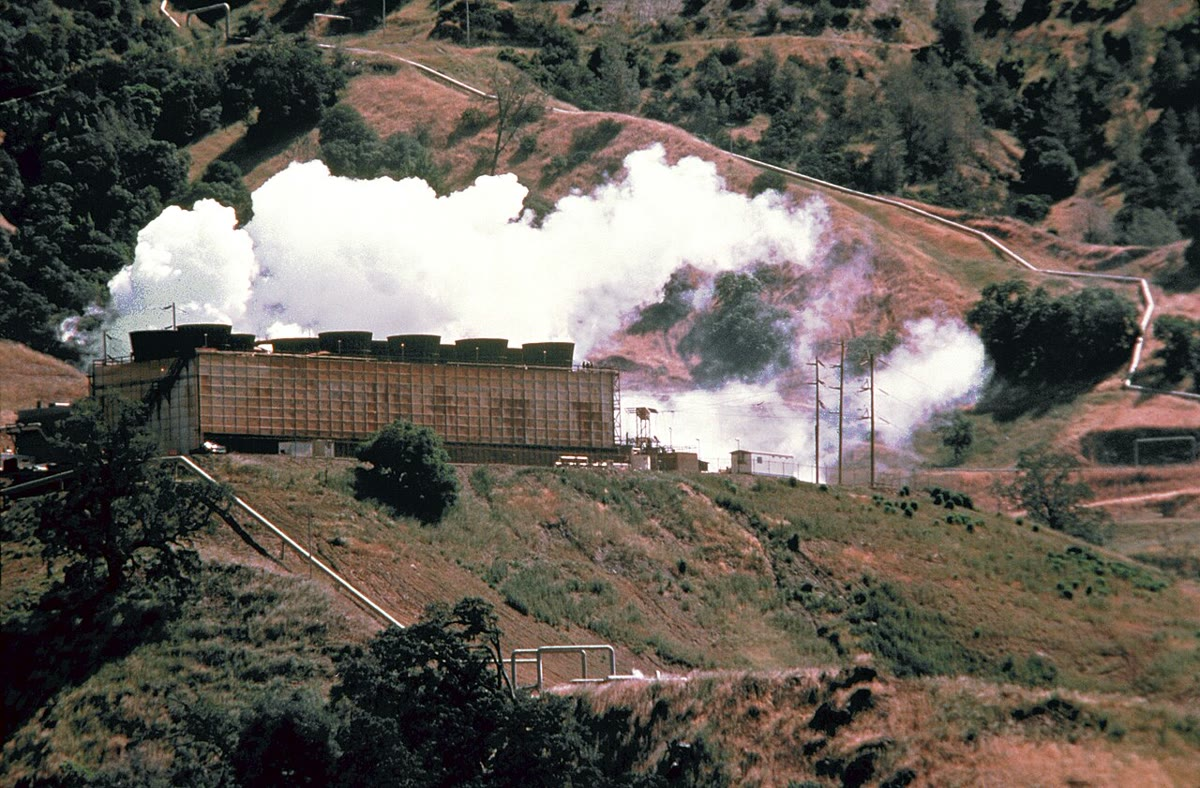
\includegraphics[width=\linewidth]{images/book4/b2-30-geyserville.jpg}
\end{minipage}
\par\smallskip{\small Left: a high-enthalpy \omterm{def:b2:energy-geology:geothermal}{geothermal system} (schematic, not to scale): water
recharged at the margins (blue) is heated over an intrusion and rises through a fractured reservoir
(red) to a hot spring; wells tap the reservoir. Right: a geothermal power plant near Geyserville,
California, in 1982, with steam pipelines on the hillside. Photograph: U.S. Department of Defense
(public domain).}
\end{omfigure}
% ledger: photo:b2-30-geyserville, usgs08g:egs

\begin{definition}[Induced seismicity]\label{def:b2:energy-geology:induced}
\emph{Induced seismicity}\index{induced seismicity} is earthquake activity caused by human
operations that change the stress or the pore-fluid pressure in the crust, most often the
injection of fluid into the ground.
\end{definition}

The mechanism is the Coulomb criterion with pore-fluid pressure: a fault slips when the shear stress
reaches $\mu(\sigma_n - p)$, so raising $p$ brings a fault that is already stressed toward failure
without any change of the tectonic load. In the 1960s, waste fluid injected into fractured
Precambrian basement beneath the Rocky Mountain Arsenal near Denver, at depths of 3.7 to
\qty{7.0}{km}, triggered earthquakes; they were confined to the part of the reservoir where the
pressure had risen by more than \qty{32}{bar} (\qty{3.2}{MPa}). The steep rise in the earthquakes
of Oklahoma has been attributed to the disposal of wastewater: four high-volume
wells could account for a fifth of the seismicity of the central United States, triggering
earthquakes more than \qty{30}{km} away. Stimulating an EGS reservoir raises the pore pressure in the
same way, by design.
% ledger: hb81:denver, keranen:oklahoma, usgs08g:egs

\section{Uranium}\label{sec:b2:energy-geology:uranium}

Two \omterm{def:b2:ore-deposits:types}{ore-deposit types} illustrate how uranium is concentrated: one at an ancient unconformity, the
other in sandstone.

\begin{definition}[Unconformity-related and roll-front uranium deposits]\label{def:b2:energy-geology:uranium}
An \emph{unconformity-related uranium deposit}\index{unconformity-related uranium deposit} is a body
of pitchblende and uraninite filling fractures and breccias in metamorphosed carbonaceous pelites and
in the quartz arenites above them, below, above or across an unconformity between Early and Middle
\omterm{def:b2:precambrian-earth:eons}{Proterozoic} rocks in an \omterm{def:b2:basins-compared:types}{intracratonic basin}. A \emph{roll-front uranium deposit}\index{roll-front
uranium deposit} is a crescent-shaped body of uranium minerals that cuts across the bedding of a
feldspathic or tuffaceous sandstone at the boundary between oxidized and reduced ground, where
uranium was deposited in a locally reduced environment, among pyrite.
\end{definition}

The unconformity deposits are hosted by rocks of 1800 to \qty{1200}{\Ma}, the metamorphosed
pelites below the unconformity and the unmetamorphosed sandstones above it; their host rocks are chloritized, and the graphitic schists that
accompany many of them are strong electrical conductors, a target for electromagnetic surveys. Key
Lake, Cluff Lake and Rabbit Lake in Saskatchewan and Jabiluka and Ranger in northern Australia are
examples. The roll fronts are younger, mostly Tertiary: in sandstones fed by felsic volcanic ash or
granite, oxidized iron minerals lie up-dip of the front and reduced ones down-dip, as in the basins
of Wyoming and the Texas Gulf Coast.
% ledger: b1693:unconformity, b1693:sandstone

\begin{proposition}[Uranium-235 in the past]\label{prop:b2:energy-geology:u235}
Let $r_0$ be today's atomic ratio $^{235}$U/$^{238}$U and $\lambda_5$, $\lambda_8$ the decay
constants of the two isotopes. A time $t$ ago the ratio was
\begin{equation}
r(t) = r_0\,e^{(\lambda_5 - \lambda_8)\,t} ,
\label{eq:b2:energy-geology:u235}
\end{equation}
and $^{235}$U made up a fraction $r/(1 + r)$ of the atoms of uranium, neglecting the trace of
$^{234}$U.
\end{proposition}

\begin{proof}
Each isotope decays exponentially: $N_5(\text{now}) = N_5(t)\,e^{-\lambda_5 t}$ and $N_8(\text{now})
= N_8(t)\,e^{-\lambda_8 t}$. Dividing, $r_0 = r(t)\,e^{-(\lambda_5 - \lambda_8)t}$.
\end{proof}

With $\lambda_5 = \qty{9.8485e-10}{yr^{-1}}$, $\lambda_8 = \qty{1.55125e-10}{yr^{-1}}$ and today's
abundances \qty{0.7204}{\percent} and \qty{99.2742}{\percent}, $r_0 = 0.0072567$; \qty{2.0}{\Ga}
ago $r = 0.0381$ and natural uranium held \qty{3.67}{\percent} of $^{235}$U, five times today's
share.
% ledger: amherst:constants, iaea:isotopes
% values: r 0.038144, 3.6743 % (calc/ch30.py)

\begin{history}[A reactor two billion years old]
In 1972, French scientists measuring uranium ore found small but significant deficits of
$^{235}$U, which they traced to the Oklo mine in Gabon. There, pods of rock held up to
\qty{65}{\percent} uranium with as little as half the normal share of $^{235}$U, and neodymium
depleted in its primordial isotope $^{142}$Nd but enriched in the isotopes 143 to 150 that fission
produces: chain reactions had run in the ore about two billion years ago, at about \qty{300}{bar}
and 400 to \qty{500}{\celsius}. Sixteen such natural reactors are known at Oklo and nearby
Bangombé, the only two deposits in the world where they have been found; organic matter had helped
concentrate the uranium, and the uranium oxide has held most of the actinides and of the
non-volatile fission products in place ever since.
\end{history}
% ledger: oklo:curtis, oklo:cowan, oklo:gl96, oklo:nagy

\section{Geological storage of carbon dioxide}\label{sec:b2:energy-geology:ccs}

\begin{definition}[Geological \ce{CO2} storage, trapping mechanisms, storage efficiency factor]\label{def:b2:energy-geology:ccs}
\emph{Geological \ce{CO2} storage}\index{geological CO$_2$ storage} is the injection of carbon
dioxide into porous rock formations deep underground, depleted oil and gas reservoirs, deep saline
formations or coal beds, for retention over long times. The \emph{\ce{CO2} trapping
mechanisms}\index{CO$_2$ trapping mechanisms} that retain it are structural (and stratigraphic)
trapping below a seal; residual trapping, as an immobile phase held in the pores by capillary
forces; solubility trapping, by dissolution in the formation water; mineral trapping, by reaction
with minerals into carbonates; and, in coal and shale, adsorption onto organic matter. The \emph{storage efficiency factor}\index{storage
efficiency factor} $E$ of a formation is the fraction of its pore volume that the injected
\ce{CO2} can be expected to fill.
\end{definition}
% ledger: srccs:retention, netl08:saline

Carbon dioxide is a gas at the surface, but its critical point lies at \qty{31.0}{\celsius} and
\qty{7.38}{MPa}. Along a geotherm of \qty{25}{\celsius\per\km} from \qty{15}{\celsius} under
hydrostatic pressure, the temperature passes the critical value at \qty{641}{m} and the pressure at
\qty{742}{m}; the density of pure \ce{CO2} jumps from \qty{234}{kg.m^{-3}} at \qty{700}{m} to
\qty{583}{kg.m^{-3}} at \qty{900}{m}, then levels off near 670 to \qty{700}{kg.m^{-3}} below
\qty{1.5}{km}. A tonne occupies \qty{534}{m^3} at the surface and \qty{1.6}{m^3} at \qty{1000}{m},
330 times less; this is why storage assessments consider only formations deeper than
\qty{800}{m}.
% ledger: nist:co2-critical, data:b4-co2-density, srccs:density, netl08:saline
% values: z_tc 641.2 m, z_pc 742.2 m; volume ratio 331.9 (figdata co2_density.py numbers)

\begin{omfigure}
\centering
\begin{minipage}[b]{0.49\linewidth}\centering
\begin{tikzpicture}
\begin{axis}[omrecord, width=0.95\linewidth, height=5.2cm, xmin=0, xmax=750, ymin=0, ymax=3,
  y dir=reverse, xlabel={density of \ce{CO2} (\unit{kg.m^{-3}})}, ylabel={depth (km)},
  tick label style={font=\scriptsize}, label style={font=\small}]
% computed in figdata/bachelor-2/co2_density.py part profile; ledger: data:b4-co2-density
\addplot[black!45, densely dashed] coordinates {(0,0.742) (750,0.742)};
\node[font=\tiny, text=black!60, anchor=south east] at (axis cs:745,0.73) {critical pressure};
\addplot[omDef, line width=1.1pt, mark=*, mark size=0.9pt] table[x=rho, y expr=\thisrow{depth_m}/1000] {figdata/out/bachelor-2-co2_density-profile.dat};
\end{axis}
\end{tikzpicture}
\end{minipage}\hfill
\begin{minipage}[b]{0.49\linewidth}\centering
\begin{tikzpicture}
\begin{axis}[width=0.95\linewidth, height=5.2cm, xmin=0, xmax=4, ymin=0, ymax=100,
  axis x line=bottom, axis y line=left, axis line style={-}, axis on top,
  xlabel={time after injection (years)}, ylabel={share of the stored \ce{CO2}},
  xtick={0,1,2,3,4}, xticklabels={1,10,100,1000,$10^4$}, ytick=\empty,
  tick label style={font=\scriptsize}, label style={font=\small}]
% schematic, after IPCC SRCCS (2005) Figure 5.9; ledger: srccs:trapping
% bands from the bottom: mineral, solubility, residual, structural (cumulative tops 0/0/1/5/15,
% 2/8/21/40/60, 10/30/56/80/90, 100)
\fill[omLithLime!60!black] (axis cs:0,0) -- (axis cs:1,0) -- (axis cs:2,1) -- (axis cs:3,5) -- (axis cs:4,15) -- (axis cs:4,0) -- cycle;
\fill[omDef!40] (axis cs:0,0) -- (axis cs:1,0) -- (axis cs:2,1) -- (axis cs:3,5) -- (axis cs:4,15) -- (axis cs:4,60) -- (axis cs:3,40) -- (axis cs:2,21) -- (axis cs:1,8) -- (axis cs:0,2) -- cycle;
\fill[omProp!40] (axis cs:0,2) -- (axis cs:1,8) -- (axis cs:2,21) -- (axis cs:3,40) -- (axis cs:4,60) -- (axis cs:4,90) -- (axis cs:3,80) -- (axis cs:2,56) -- (axis cs:1,30) -- (axis cs:0,10) -- cycle;
\fill[black!15] (axis cs:0,10) -- (axis cs:1,30) -- (axis cs:2,56) -- (axis cs:3,80) -- (axis cs:4,90) -- (axis cs:4,100) -- (axis cs:0,100) -- cycle;
\node[font=\scriptsize] at (axis cs:1.1,72) {structural};
\node[font=\scriptsize] at (axis cs:2.1,38) {residual};
\node[font=\scriptsize] at (axis cs:3.1,22) {solubility};
\node[font=\scriptsize, text=white, anchor=south east] at (axis cs:3.98,0.5) {mineral};
\end{axis}
\end{tikzpicture}
\end{minipage}
\par\smallskip{\small Left: density of pure \ce{CO2} with depth along a geotherm of
\qty{25}{\celsius\per\km} from \qty{15}{\celsius}, under hydrostatic pressure. Data: NIST Chemistry
WebBook (Span--Wagner equation of state), along the conditions of the IPCC Special Report on Carbon
Dioxide Capture and Storage (2005). Right: how the trapping mechanisms share the stored \ce{CO2}
over time (schematic, after the same report): trapping by the seal gives way to the residual,
dissolved and mineral forms, which are less mobile.}
\end{omfigure}

\begin{proposition}[Storage capacity of a formation]\label{prop:b2:energy-geology:capacity}
A formation of area $A$, thickness $h$ and porosity $\phi$, in which \ce{CO2} has the density $\rho$
and the \omterm{def:b2:energy-geology:ccs}{storage efficiency factor} is $E$, can store the mass
\begin{equation}
M = A\,h\,\phi\,\rho\,E .
\label{eq:b2:energy-geology:capacity}
\end{equation}
For a depleted oil field that has produced a stock-tank volume $N_p$, replacing the produced oil
volume for volume gives $M = \rho\,N_p\,B_o$.
\end{proposition}

\begin{proof}
The pore volume is $Ah\phi$, of which the \ce{CO2} fills a fraction $E$, at density $\rho$. In the
oil field, the produced oil occupied $N_pB_o$ in the reservoir, the volume the \ce{CO2} takes over.
\end{proof}

For deep saline formations, simulations give $E$ between 1 and \qty{4}{\percent} of the pore volume
over a 15 to 85 per cent confidence range, with a median near \qty{2}{\percent}: most of the pore
space is never reached, or keeps its water. A formation of \qty{1000}{km^2}, \qty{50}{m} thick and of
porosity 0.20 at \qty{2000}{m} ($\rho = \qty{686}{kg.m^{-3}}$) stores \qty{137}{Mt} at $E =
\qty{2}{\percent}$.
% ledger: netl08:saline, data:b4-co2-density
% values: 1e9*50*0.2*686*0.02 = 1.372e11 kg (calc/ch30.py)

Once injected, the \ce{CO2} rises under the seal and spreads. Behind the migrating plume, capillary
forces hold residual saturations that may reach 15 to \qty{25}{\percent} of the pore space;
dissolution takes up 20 to \qty{60}{kg} of \ce{CO2} per cubic metre of formation water, and in
slowly flowing formations up to \qty{30}{\percent} of the injected \ce{CO2} dissolves within tens of
years. Solubility trapping dominates over tens to hundreds of years, ionic forms over hundreds to
thousands, mineral trapping over thousands to millions: reactions with carbonate minerals take days,
with silicates hundreds to thousands of years. The storage becomes more secure as it ages, and at
well-chosen and well-managed sites the retention of \qty{99}{\percent} or more of the \ce{CO2} over
1000 years was judged likely.
% ledger: srccs:trapping, srccs:retention

\begin{dated}{2005}
At Sleipner, in the North Sea about \qty{250}{km} off Norway, the \ce{CO2} separated from the
natural gas of the field, about \qty{9}{\percent} of it, has been injected since October 1996 into
the Utsira formation, an unconsolidated saline sandstone 800 to \qty{1000}{m} below the sea floor,
at about \qty{1}{Mt} a year. By early 2005 more than \qty{7}{Mt} had been stored, of the \qty{20}{Mt}
planned over the project's life. Repeated seismic surveys image the plume, whose footprint was then
about \qty{5}{km^2}, and show that the caprock above it seals it.
\end{dated}
% ledger: srccs:sleipner

\begin{inthefield}[Reading a well while it is drilled]
\centering
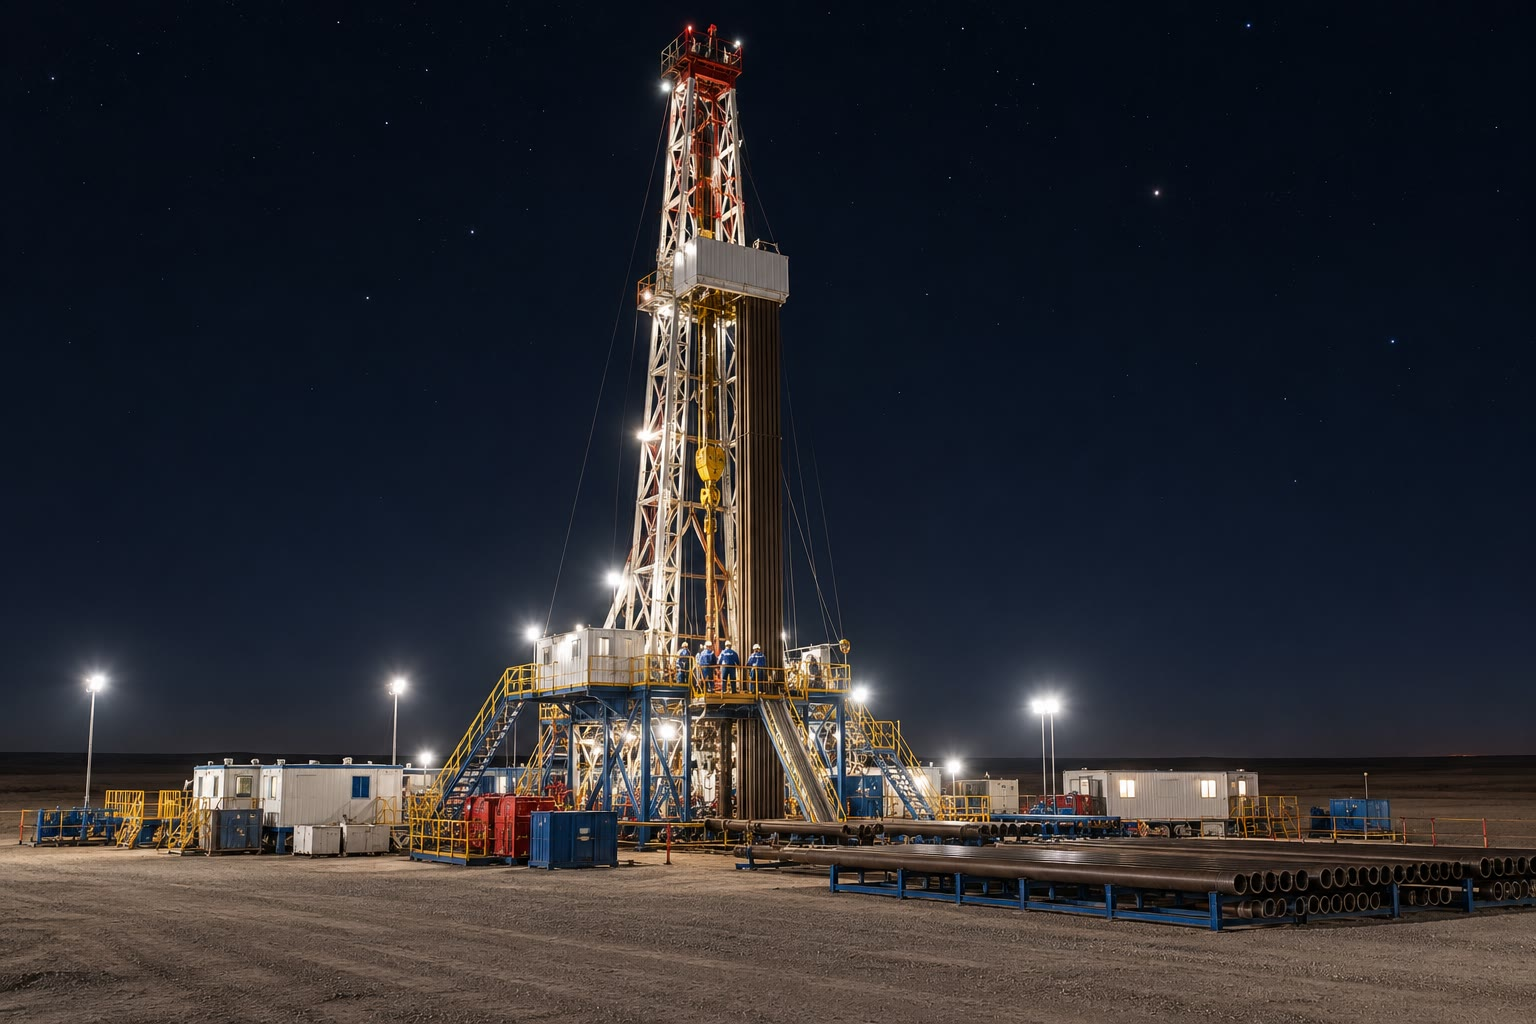
\includegraphics[width=0.56\linewidth]{images/book4/ai/b2-rig-night.jpg}
\par\smallskip{\small A land drilling rig at night (AI-generated illustration).}
\par\medskip\raggedright
When a section of a well is finished, geophysicists lower tools on a cable and record against
depth the properties of the rocks around the hole. One records their natural radioactivity, low in
sandstone and higher in shale; another their bulk density, from which the porosity follows as
(grain density $-$ bulk density)/(grain density $-$ fluid density), with \qty{2.65}{g/cm^3} for
quartz grains and about \qty{1}{g/cm^3} for the water. Read together, these borehole logs give the
net reservoir thickness and the porosity that enter the volumetric formulas of this chapter.
\end{inthefield}
% ledger: keys:gamma, keys:density-porosity

\section*{Exercises}\label{sec:b2:energy-geology:exercises}

Data for the exercises, unless stated otherwise: $R = \qty{8.314}{J.mol^{-1}.K^{-1}}$; one million
years is \qty{3.156e13}{s}; Green River kerogen $A = \qty{9.21e13}{s^{-1}}$, $E/R = \qty{26800}{K}$;
atomic masses C 12.011, H 1.008, O 15.999; density of \ce{CO2} along the profile of the figure:
\qty{1.872}{kg.m^{-3}} at the surface, 583 at \qty{900}{m}, 621 at \qty{1000}{m}, 686 at
\qty{2000}{m}. Round to three significant figures.
% ledger: codata:R, fp14:gr-daem, data:b4-co2-density

\begin{exercise}[$\star$]\label{exo:b2:energy-geology:1}
(a) Four immature kerogens have atomic H/C of 1.58, 0.95, 1.24 and 1.12. Assign each a type and say
which would yield mainly gas. (b) Check the ratios H/C and O/C of the formula
C$_{100}$H$_{150}$N$_3$O$_8$S. (c) Find them from the mass composition C \qty{77.4}{\percent}, H
\qty{9.8}{\percent}, O \qty{8.2}{\percent}.
\end{exercise}

\begin{exercise}[$\star$]\label{exo:b2:energy-geology:2}
(a) Five samples of a type~II source rock have $R_o$ = 0.45, 0.68, 1.1, 1.6 and \qty{2.5}{\percent}.
Describe the state of each with respect to oil and gas. (b) Is a type~III kerogen at $R_o =
\qty{0.68}{\percent}$ generating methane? (c) Which converted fraction $F$ of Easy\%Ro corresponds to
$R_o = 0.6$ and \qty{1.3}{\percent}?
\end{exercise}

\begin{exercise}[$\star$]\label{exo:b2:energy-geology:3}
A trap covers \qty{6}{km^2}; its reservoir has \qty{25}{m} of net thickness, porosity 0.18 and water
saturation 0.30, and $B_o = 1.25$. (a) Find the oil volume in the reservoir and the STOIIP. (b) Find
the volume produced for \omterm{def:b2:energy-geology:volumetrics}{recovery factors} of 0.30 and 0.40.
\end{exercise}

\begin{exercise}[$\star$]\label{exo:b2:energy-geology:4}
A sandstone aquifer \qty{200}{m} thick under \qty{10}{km^2} is at \qty{75}{\celsius}. (a) Find its
\omterm{def:b2:energy-geology:geothermal}{heat in place} above \qty{15}{\celsius}, with $C = \qty{2.5}{MJ.m^{-3}.K^{-1}}$. (b) To which
enthalpy class does it belong? (c) Find the mean thermal power over 30 years for $R_g = 0.25$.
\end{exercise}

\begin{exercise}[$\star\star$]\label{exo:b2:energy-geology:5}
(a) Find the activation energy for which an Arrhenius rate doubles between 100 and
\qty{110}{\celsius}. (b) By what factor does the rate of the Green River reaction grow over the same
interval? (c) Which of the two rules gives more weight to the time a rock spent at low temperature,
and what does this imply for a TTI computed for a type~I source rock?
\end{exercise}

\begin{exercise}[$\star\star$]\label{exo:b2:energy-geology:6}
(a) Show from \eqref{eq:b2:energy-geology:maturation} that the temperature of half conversion obeys
$T = (E/R)\big/\ln\bigl[A T^2/(\beta\,(E/R)\ln 2)\bigr]$, and solve it by iteration for the Green
River kerogen heated at \qty{1}{\celsius\per\Myr} and at \qty{10}{K} per minute. (b) Compare the
difference with the estimate $(RT^2/E)\ln(\beta_2/\beta_1)$ taken at the lower temperature, and
explain the discrepancy.
\end{exercise}

\begin{exercise}[$\star\star$]\label{exo:b2:energy-geology:7}
Using \eqref{eq:b2:energy-geology:u235} and the data of the text: (a) find the share of $^{235}$U in
natural uranium \qty{2.0}{\Ga} and \qty{1.8}{\Ga} ago; (b) when was it \qty{3.00}{\percent}?
(c) Oklo ore holds as little as half today's normal share of $^{235}$U. Ignoring the $^{238}$U
consumed, what fraction of the $^{235}$U present at the time of the reactions was fissioned, and
why does the later decay not change the answer?
\end{exercise}

\begin{exercise}[$\star\star$]\label{exo:b2:energy-geology:8}
(a) Find the volume of \qty{1}{Mt} of \ce{CO2} at the surface, at \qty{1000}{m} and at
\qty{2000}{m}. (b) At Sleipner more than \qty{7}{Mt} had been injected by 2005, at about
\qty{900}{m}, into a plume of footprint \qty{5}{km^2}. Taking a porosity of 0.35 and a \ce{CO2}
saturation of 0.30 in the plume, find the volume of rock it occupies and its mean thickness.
\end{exercise}

\begin{exercise}[$\star\star$]\label{exo:b2:energy-geology:9}
A high-enthalpy reservoir measures $3 \times 2 \times \qty{1.5}{km}$ at \qty{250}{\celsius}, with
$C = \qty{2.6}{MJ.m^{-3}.K^{-1}}$. (a) Find its \omterm{def:b2:energy-geology:geothermal}{heat in place} above \qty{15}{\celsius}. (b) Find the
mean thermal power over 30 years for $R_g = 0.1$ and $0.25$. (c) Its field covers \qty{6}{km^2};
at 10 to \qty{20}{MW} of electricity per square kilometre, what fraction of the thermal power at
$R_g = 0.1$ becomes electricity?
\end{exercise}

\begin{exercise}[$\star\star\star$]\label{exo:b2:energy-geology:10}
A fault at about \qty{4}{km} carries a normal stress of \qty{80}{MPa} and a shear stress of
\qty{22}{MPa}; its friction coefficient is 0.6 and the pore pressure is hydrostatic,
\qty{39}{MPa}. (a) Is the fault stable? Find the pore-pressure rise that brings it to failure, in
megapascals and in bars, and compare with the Denver threshold. (b) The same if the shear stress is
\qty{24}{MPa}. (c) Explain why earthquakes can be triggered kilometres away from an injection well,
and years after injection began.
\end{exercise}

\begin{exercise}[$\star\star\star$]\label{exo:b2:energy-geology:11}
(a) From the approximation in \eqref{eq:b2:energy-geology:maturation}, show that at a constant
heating rate the transformation ratio rises from \qty{10}{\percent} to \qty{90}{\percent} over a
temperature interval $\Delta T \approx \bigl[\ln\ln 10 - \ln\ln(10/9)\bigr]\,RT^2/E$. (b) Evaluate it
for the Green River kerogen at \qty{1}{\celsius\per\Myr}. (c) Compare with the solid curve of the
figure and explain the difference.
\end{exercise}

\begin{exercise}[$\star\star\star$]\label{exo:b2:energy-geology:12}
Sleipner is to store \qty{20}{Mt} of \ce{CO2}. (a) Find the volume of formation water needed to
dissolve it all, at 20 and at \qty{60}{kg.m^{-3}}. (b) Find its volume as a free phase at
\qty{1000}{m}. (c) With $E = \qty{2}{\percent}$, find the pore volume of formation required, and
the area of a formation \qty{50}{m} thick of porosity 0.30.
\end{exercise}
% ledger: srccs:trapping, srccs:sleipner, hb81:denver

\begin{problem}[{Weekend problem --- One basin, two uses}]\label{pb:b2:energy-geology:1}
In an invented basin, a type~I source rock was deposited at \qty{120}{\Ma} at the surface.
Sediment then accumulated at \qty{60}{m} per million years until \qty{70}{\Ma}, and at \qty{30}{m}
per million years since. The surface is at \qty{15}{\celsius} and the geotherm is steady at
\qty{25}{\celsius\per\km}. The kerogen has the Green River kinetics of the text (single energy).
Its kitchen, the mature part of the source rock, covers \qty{400}{km^2}, is \qty{50}{m} thick and
of density \qty{2400}{kg.m^{-3}}, and can yield \qty{30}{kg} of oil per tonne of rock at full
conversion; the oil has a surface density of \qty{850}{kg.m^{-3}}. The oil fills a trap of
\qty{12}{km^2} whose reservoir, centred at \qty{2000}{m}, has a net thickness of \qty{40}{m},
porosity 0.22 and water saturation 0.25, with $B_o = 1.30$. Use the data of the exercises; round to
three significant figures.

\noindent\textbf{Part I --- Burial and the time--temperature index.}
\begin{enumerate}
  \item Find the depth and temperature of the source rock at \qty{70}{\Ma} and today.
  \item Find its heating rate in each phase.
  \item Find the time it spent in each interval of \qty{10}{\celsius}, from \qty{15}{\celsius} to
        its present temperature.
  \item Compute its TTI today (method of the text).
  \item When, at what temperature and at what depth did it pass a TTI of 15?
  \item The same for 75 and 160.
  \item By the TTI, is the source rock still generating oil?
\end{enumerate}

\noindent\textbf{Part II --- Conversion by kinetics.}
\begin{enumerate}[resume]
  \item Find the rate constant at \qty{90}{\celsius} and show that less than \qty{0.2}{\percent} of
        the kerogen can have been converted before \qty{70}{\Ma}.
  \item Using \eqref{eq:b2:energy-geology:maturation} with the heating rate of the second phase,
        find the unconverted fraction and the transformation ratio today.
  \item Find the temperature of half conversion at this heating rate (exercise~\ref{exo:b2:energy-geology:6}).
  \item When was it reached?
  \item Compare with the time of peak generation given by the TTI, and explain the difference.
  \item Would a type~II kerogen with a lower mean activation energy have converted earlier or later?
\end{enumerate}

\noindent\textbf{Part III --- Oil generated, in place and recoverable.}
\begin{enumerate}[resume]
  \item Taking a transformation ratio of 0.92, find the mass of oil generated in the kitchen.
  \item Find its volume at the surface.
  \item Find the STOIIP of the trap.
  \item What fraction of the oil generated does the trap hold? Keep \qty{1.56e9}{m^3} for (15).
  \item Find the oil produced for a \omterm{def:b2:energy-geology:volumetrics}{recovery factor} of 0.35.
  \item Why is the \omterm{def:b2:energy-geology:volumetrics}{recovery factor} much less than one, and what would injecting \ce{CO2} change?
\end{enumerate}

\noindent\textbf{Part IV --- The depleted field as a \ce{CO2} store.}
\begin{enumerate}[resume]
  \item Find the temperature and hydrostatic pressure of the reservoir. Is injected \ce{CO2}
        supercritical there? Read its density on the figure.
  \item Keeping $N_p = \qty{2.13e7}{m^3}$, find the reservoir volume freed by production.
  \item Express it as a \omterm{def:b2:energy-geology:ccs}{storage efficiency factor} of the pore volume of the trap, and compare with
        saline formations.
  \item A saline formation below the field covers \qty{600}{km^2}, is \qty{80}{m} thick, of
        porosity 0.20, with \ce{CO2} at \qty{691}{kg.m^{-3}}. Find its capacity at $E =
        \qty{2}{\percent}$.
  \item How many years of injection at the Sleipner rate would fill it?
  \item With $\rho = \qty{686}{kg.m^{-3}}$ and the freed volume rounded to \qty{2.77e7}{m^3}, find
        the \ce{CO2} storage capacity of the depleted reservoir, in megatonnes.
\end{enumerate}
\end{problem}
% ledger: fp14:gr-daem, waples80:tti, hamm14:tti-table, netl08:oilgas, netl08:saline, data:b4-co2-density, nist:co2-critical, srccs:sleipner
